\section{Main Window}
\label{sec:ui_main_window} 

When the application is started for the first time, the main window is shown as follows. 

\begin{figure}[H]
  \hspace*{-2.5cm}
    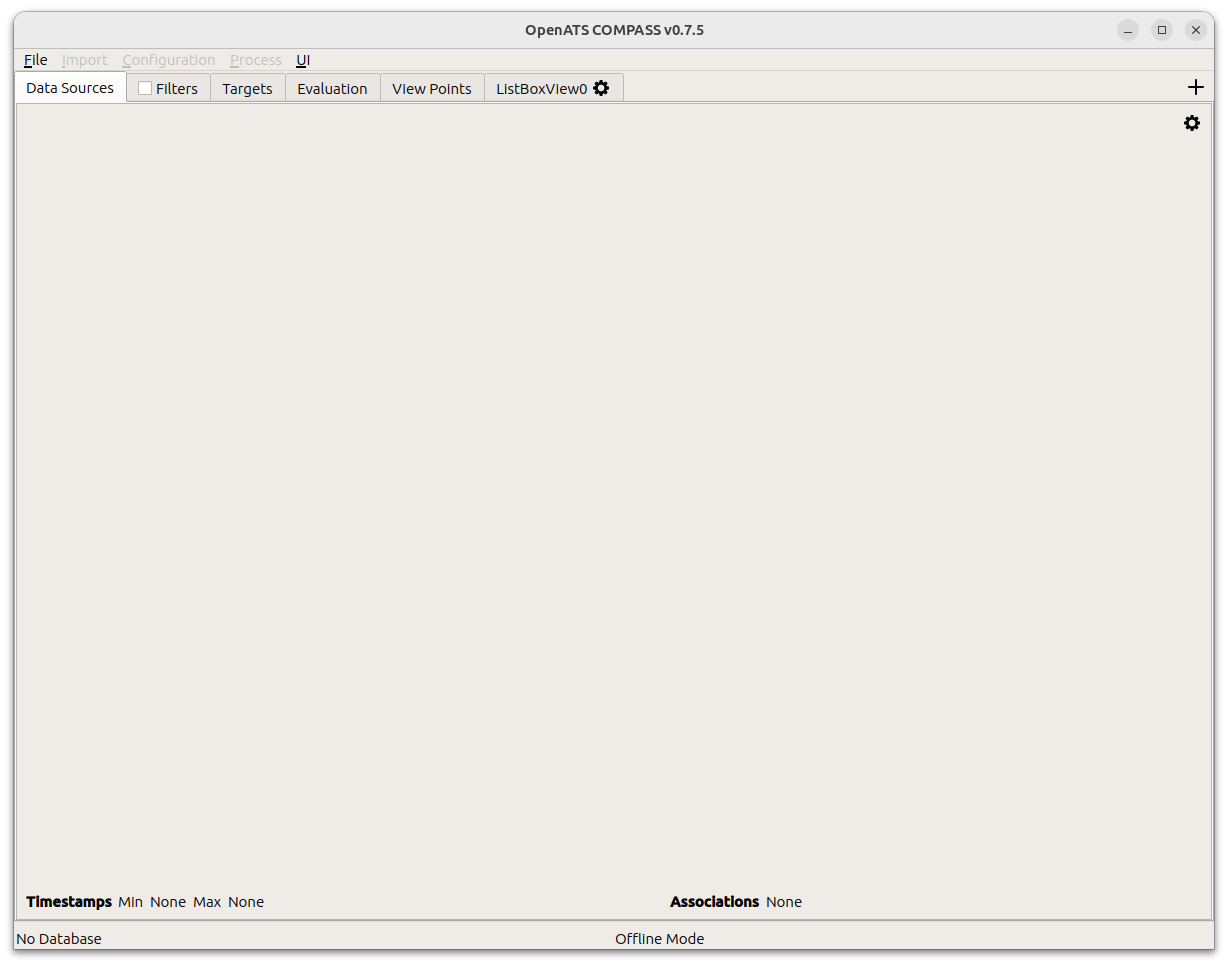
\includegraphics[width=19cm]{figures/main_window.png}
  \caption{Main Window}
\end{figure}

In the simplest use case, the main menubar allows to open or create a database and importing data. 
After this step, data of interest can be chosen using the main tab area, and loaded from the database using the 'Load' button in the main statusbar. \\

The loaded data is then shown in Views located either in the main tab area or in other windows. \\

The values set in the 'Data Sources' and 'Filter' tabs define the dataset loaded from the database into memory (RAM). Only the data required by the application is loaded into memory.\\

Only one dataset can exist at a time. At the beginning of a loading process, the old dataset is cleared, and a new one is filled sequentially from the database. This single dataset is then distributed to all existing views. \\

When new Views are added, or Views require additional data, a manual re-load has to be performed by the user. \\

To close the application either the 'File' menu can be used, or the close button in the main window decoration. \\

Please \textbf{note} that using the close button in windows other than the main window only removes the respective Views, but does not close the application.

Please \textbf{note} that depending on the application status some parts of the UI are inaccessible, e.g. are only available when a database was opened.

\subsection{Main Menubar}

A common workflow is to open or create a database using the 'File' menu. If new data is to be imported, this can be done using the 'Import' menu. 
After all data was imported, the 'Process' menu can be used to post-process the data (if desired). \\

At the top exists a main menubar, which allows access to the following groups:

\begin{itemize}
 \item \nameref{sec:ui_overview_file_menu}: Open/close a database, quit application
 \item \nameref{sec:ui_overview_import_menu}: Import ASTERIX, NMEA data
 \item \nameref{sec:ui_overview_config_menu}: Configure data sources, sectors
 \item \nameref{sec:ui_overview_process_menu}: Various processing tasks for imported data
 \item \nameref{sec:ui_overview_ui_menu}: Reset Views
\end{itemize}
\  \\

\subsection{Main Tab Area}

When a database was opened and data was imported into it, the main tab area allows configuration of what data should be loaded using the 'Data Sources' and 'Filter' tabs. 
Additional main features are also located here (e.g. 'Evaluation' and 'View Points'). Multiple Views can be added as additional tabs. \\

The following tabs can exist in the main tab area:
\begin{itemize}
 \item Data Sources: Select which data sources and lines should be loaded
  \begin{itemize}
 \item see \nameref{sec:ui_data_sources}
 \end{itemize}
 \item Filter: Filter which data should be loaded
   \begin{itemize}
 \item see \nameref{sec:ui_filters}
 \end{itemize}
  \item Targets: After calculation of unique targets, the created targets are shown
 \begin{itemize}
 \item see \nameref{sec:ui_targets}
 \end{itemize}
 \item Evaluation: Allows adapting/defining requirement-based standards and compliance assessment of said standards
 \begin{itemize}
 \item see \nameref{sec:eval}
 \end{itemize}
 \item View Points: Show/edit specific cases saved as View Points
  \begin{itemize}
 \item see \nameref{sec:view_points}
 \end{itemize}
 \item Views: All views included in the main window, e.g. TableView0
\end{itemize}
\  \\

To add additional views, the \includegraphics[width=0.5cm,frame]{../../data/icons/crosshair_fat.png} button can be used. 
Views can be added either to the window in which the button was clicked ('Add Here') or in a new window ('Add In New Window'). \\

A single View can be removed by clicking the \includegraphics[width=0.5cm,frame]{../../data/icons/edit.png} button in its tab (next to the Views name) and selecting 'Close'. \\

Please \textbf{note} that using the close button in windows other than the main window only removes the respective Views, but does not close the application.

%Right of the tabs, the 'Add View' button \includegraphics[width=0.5cm,frame]{../../data/icons/crosshair_fat.png} is located. It can be clicked to add additional views to the current window or in a new window. \\

%\paragraph{Main Tabs}
%The 'Data Sources' tab shows which data sources exist in the database. \\

%The 'Evaluation' tab allows adapting/defining requirement-based standards  and compliance assessment of said standards. For more information please refer to \nameref{sec:eval}. \\

%The 'View Points' tab shows view points and allows for associated functions. For more information please refer to \nameref{sec:view_points}.

\subsection{Main Statusbar}

The main statusbar at the bottom shows general information and contains the 'Load' button used to trigger a loading process (only visible when database was opened). \\

The following information is shown:

\begin{itemize}
 \item Database indicator: Shows 'No Database' or currently opened database file name
 \item Application mode: 'Offline' or 'Live'
\end{itemize}
\  \\






